\subsection{Randomness Beacon Architecture}

As defined by NIST, a \textbf{Randomness Beacon} is a service that provides periodic pulses of random numbers. These pulses are timestamped, hash-chained, and signed~\cite{kelsey2019}.

A beacon is composed of:
\begin{itemize}
    \item An \textbf{engine}, a computer with clear physical boundaries where pulses are formed and the beacon app runs.
    \item A \textbf{frontend} providing access to the latest pulse and history of all pulses generated.
    \item An \textbf{HSM} (Hardware Security Module), independent from the engine, used for cryptographic operations.
    \item At least \textbf{two RNGs}, with at least one being independent from the beacon's engine.
\end{itemize}

\begin{figure}[h]
    \centering
    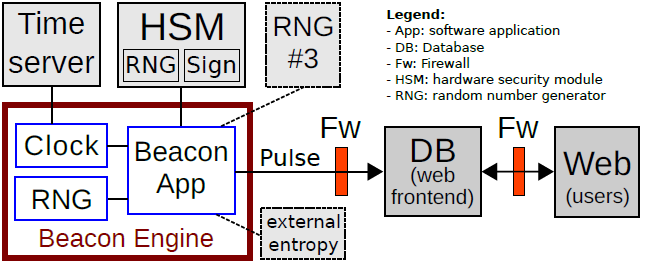
\includegraphics[width=\columnwidth]{images/ArchitectureNISTBeacon.PNG}
    \caption{The general layout of a Randomness Beacon~\cite{kelsey2019}.}
    \label{fig:beacon-architecture}
\end{figure}

The \textbf{NIST Randomness Beacon} produces a 512-bit pulse every minute and makes it publicly available with a timestamp. The beacon currently uses three RNGs:
\begin{itemize}
    \item The Intel RNG included in the engine,
    \item A QRNG based on photon detection developed by NIST,
    \item The hardware RNG inside the HSM~\cite{kelsey2018}.
\end{itemize}

\subsection{The Intel RNG}

The Intel RNG is a DRNG integrated into many Intel CPUs. It utilizes the \texttt{RDRAND} and \texttt{RDSEED} instructions, which are part of the Intel 64 architecture, and implements them directly in hardware. Its architecture includes an entropy source, a conditioner to convert entropy into random numbers, and two parallel outputs: a DRBG and an ENRNG~\cite{mechalas2018}.

\begin{figure}[h]
    \centering
    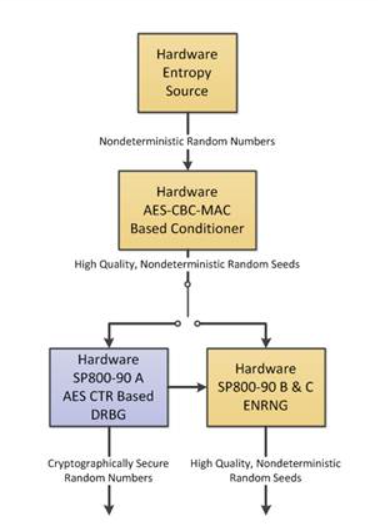
\includegraphics[width=\columnwidth]{images/IntelDRNPipeline.PNG}
    \caption{Intel’s DRNG Component Architecture~\cite{mechalas2018}.}
    \label{fig:intel-drng-architecture}
\end{figure}

The entropy source measures thermal noise within the silicon of the CPU and outputs randomness as a binary stream at a rate of 3 GHz.

\subsection{The QRNG Based on Photon Detection}

The QRNG based on photon detection is described by Zhang et al.~\cite{zhang2021}. It operates as follows:

\begin{quote}
At each trial, a horizontally polarized single photon is emitted from a source, and then measured randomly along either the X-basis (diagonal/anti-diagonal polarization basis) to generate a random bit or the Z-basis (horizontal/vertical polarization basis) to verify the prepared state.
\end{quote}

In practice, the NIST QRNG measures photons prepared in a superposition of two time bins---early ($t_e$) and late ($t_l$)---using \textbf{time-bin encoding}. Photons pass through an unbalanced Mach-Zehnder interferometer (MZI), where the path-length difference matches the separation between $t_e$ and $t_l$. Detection times correspond to:
\begin{itemize}
    \item $t_e$ or $t_l$: no interference (Z-basis measurement)
    \item $t_m$: interference (X-basis measurement)
\end{itemize}

The basis choice is passive and random, depending on the photon's path through the MZI. Outcomes are fundamentally unpredictable due to quantum mechanics, ensuring certifiable quantum randomness.

\subsection{Hashing of RNG Output}

The NIST Randomness Beacon concatenates outputs from its RNGs and applies a SHA-512 hash. The resulting hash is the \textit{localRandomValue} of the pulse~\cite{kelsey2021}.

\subsection{CTR\_DRBG: Counter Mode Deterministic Random Bit Generator}
\label{sec:counter_mode_deterministic_random_bit_generator}

\begin{quote}
\textbf{CTR\_DRBG} is a standardized deterministic random bit generator built from a block cipher operating in counter (CTR) mode, as defined in NIST SP 800-90A~\cite{nist80090a}. It transforms a secure symmetric cipher (e.g., AES) into a cryptographically strong pseudorandom bit source. The counter mode ensures each block is unique by incrementing a counter for each output, preventing repetition under the same key and seed. This construction is widely used in cryptography for generating keys, IVs, and session tokens.
\end{quote}


\subsection{Random Number Generation}
\label{sec:random_generation}

\noindent
For this exercise, three different forms of random number generation were performed. The first was through the \textit{CTR\_DRBG} algorithm, which used random keys generated by the \texttt{random} function of the Python programming language version 3.9 as seeds and was executed on a MacBook Pro M3 Pro computer. This detail may lead to different results if the experiment is replicated. However, we assume that Python's \texttt{random} function generates a uniform randomness distribution, simulating an entropic system for generating random bits.

For the second option, a sequential range of seeds was chosen, which were formatted in 32 bits to ensure compatibility with AES encryption. The sequence started at 1 and increased by one until reaching 50 million seeds. These seeds were then used to execute the \textit{CTR\_DRBG} algorithm, which generates the pseudo-random bit values.

The third approach made use of the Beacon system. In this case, the official NIST API was consumed to retrieve the last 15,600 random bits, generated from 512-bit values, obtained from the historical records maintained by the system.


\section{CTR\_DRBG Counter mode Deterministic Random Bit Generator}
\label{sec:ctr_drbg}

\begin{quote}
\textbf{CTR\_DRBG (Counter mode Deterministic Random Bit Generator)} is a standardized method for constructing a deterministic random bit generator (PRNG) using a block cipher operating in counter (CTR) mode. This technique is defined in NIST Special Publication 800-90A, titled \textit{``Recommendation for Random Number Generation Using Deterministic Random Bit Generators''}. Essentially, CTR\_DRBG transforms a secure symmetric cipher---such as AES---into a cryptographically strong source of pseudorandom bits. The counter mode ensures that each generated block is unique by systematically incrementing a counter value for each new data request, thus preventing the repetition of output sequences under the same key and seed. This approach is widely used in cryptographic applications requiring high security and reliability in random data generation, such as key generation, initialization vectors, and session tokens.
\end{quote}

\subsection*{How It Works}

The internal state of the CTR\_DRBG consists of two components:

\begin{itemize}
    \item \textnormal{\textbf{V}}: A state vector that acts as a counter.
    \item \textnormal{\textbf{Key}}: A symmetric encryption key (commonly 128 or 256 bits).
\end{itemize}

To generate random output, the algorithm encrypts sequential values derived from \texttt{V} using the current \texttt{Key}. For each block of output, the counter \texttt{V} is incremented. 

A secure seed—typically composed of entropy input, a nonce, and optional personalization string—is required to properly initialize the internal state.

\textit{CTR\_DRBG} utilizes an approved block cipher algorithm in counter (CTR) mode, as described in \cite{nist80090a}. Unlike the standard CTR mode, it allows the counter field to occupy only a portion of the cipher input block, as specified in \cite{nist80038d}.

For context, the block size depends on the cipher: 64 bits for TDEA and 128 bits for AES. The same block cipher algorithm and key length are used consistently throughout all encryption operations in the DRBG. These parameters must meet or exceed the required security level of the intended application.

The construction of \textit{CTR\_DRBG} revolves around an internal update function, \texttt{CTR\_DRBG\_Update}, illustrated in Figure~\ref{fig:ctr_drbg_update}. This function is invoked during instantiation, reseeding, and random bit generation to update the internal state using newly provided entropy or additional input. It also ensures that the internal state changes appropriately after every generation step.

Figure~\ref{fig:ctr_drbg_stages} outlines the full operation of \textit{CTR\_DRBG} in three stages: instantiation, generation, and reseeding.

\begin{figure}[htbp]
    \centering
    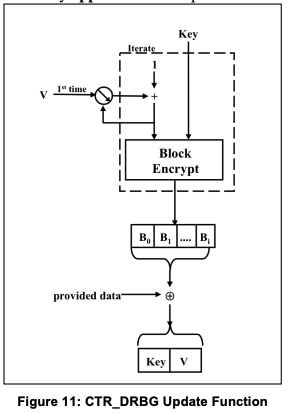
\includegraphics[width=0.9\linewidth]{images/Figure11_CTR_DRBG_Update_Function.png}
    \caption{CTR\_DRBG Update function as shown in \cite{nist-sp800-90a}.}
    \label{fig:ctr_drbg_update}
\end{figure}

\begin{figure}[htbp]
    \centering
    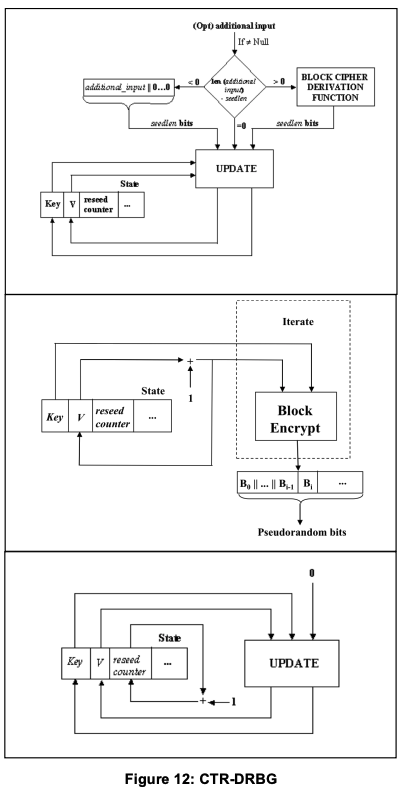
\includegraphics[width=0.9\linewidth]{images/Figure12_CTR_DRBG.png}
    \caption{The three stages of CTR\_DRBG operation as illustrated in \cite{nist-sp800-90a}.}
    \label{fig:ctr_drbg_stages}
\end{figure}


To provide an overview of what can be found in the source article, we can say that \textit{CTR\_DRBG} is a deterministic random bit generator that uses an approved symmetric encryption algorithm, such as AES, in counter (CTR) mode to produce secure random bits. Its internal state consists of a counter vector called \texttt{V} and a secret key, \texttt{Key}, which are updated through an internal function named \texttt{CTR\_DRBG\_Update} during instantiation, generation, and reseeding, thus ensuring the cryptographic security of the generator. At each step, \texttt{V} is encrypted with \texttt{Key} and incremented to generate non-repeating pseudorandom blocks. It requires a secure initial seed with sufficient entropy to avoid predictability and can be periodically reseeded to maintain long-term security. This flexible design allows for the use of variable block sizes and key lengths depending on the algorithm (e.g., 128 bits for AES) and meets robust cryptographic standards, making it reliable for applications that require secure random number generation.

\subsection{AES - Advanced Encryption Standard}
\label{sec:aes}
\begin{quote}
\textbf{AES (Advanced Encryption Standard)} is a symmetric encryption algorithm widely used across various applications for securing data. It was established by the National Institute of Standards and Technology (NIST) in 2001 as a replacement for the older Data Encryption Standard (DES). AES operates on fixed-size blocks of data (128 bits) and supports key sizes of 128, 192, or 256 bits, providing a high level of security against brute-force attacks. The algorithm employs a series of transformations, including substitution, permutation, and mixing, to encrypt plaintext into ciphertext and vice versa. Its efficiency and robustness have made it the de facto standard for encryption in many cryptographic protocols and systems.
\end{quote}


\subsection{Seeds obtaining and random bits generation}
\label{sec:seeds_obtaining_random_bits_generation}

\subsection{Distribution of Random Bits Generated with Python Random Seeds}
\label{sec:distribution_python_seed}

The distribution results of each technique are separated by the method used to obtain the seed versus the technique used to distill and obtain the random big number, so we can observe different results for each case.

To view the distribution of values, distribution graphs were used, either standard or uniform, depending on the input data. In our experiments, uniform distributions were shown. 8-bit segments were taken, dividing the entire input data set into byte blocks, obtaining bytes from 0 to 255. This range of possibilities gives us a visual of how the results are distributed.

We begin with the first technique, which was the generation of 6.25 million 32-byte seeds that were used to generate 6.25 million random bytes, or 50 million random bits, using the \textit{CTR\_DRBG} technique. The graph we see below leads us to the conclusion that there is a uniform distribution of the results without pronounced peaks, which are a symptom of an effective system in generating random bits.


\subsection{Distribution of Random Bits Generated with Sequential Seeds}
\label{sec:distribution_sequential_seed}

For the following test, sequential seeds were used starting at 1 and reaching 6.5 million in the set of natural numbers. This number was converted to binary and turned into a 32-bit number, then it was used as a seed to generate the distribution with the \textit{CTR\_DRBG} method, showing a uniform distribution without much variation. Unexpectedly, it is seen that the distribution behaves very similar to obtaining reliable seeds with true entropy.


\subsection{Distribution from the NIST Beacon}
\label{sec:distribution_nist_beacon}
Finally, we reported the Beacon, and this time we used the official NIST API, where we downloaded a history of just over 15,600 pulses. Each pulse corresponds to a hexadecimal message that corresponds to a 512-bit random number, which allowed us to generate the histogram and create the tests.

\subsection{Quantum Random Number Generator}

Quantum Random Number Generation (QRNG) harnesses the inherent indeterminacy of quantum mechanics to produce random sequences theoretically unpredictable by classical means. At its core, QRNG utilizes qubits which, through the principle of superposition, can represent multiple states simultaneously until a measurement is performed. This act of measurement is pivotal, compelling a qubit to collapse from its superposition into a definite classical state (0 or 1), with the specific outcome governed by quantum probabilities, forming the basis of true randomness.
The translation of these quantum mechanical principles into a practical random bit stream involves a carefully orchestrated process. It begins with the precise preparation of quantum states specifically designed to maximize outcome uncertainty. Subsequent interactions with these prepared states, followed by their measurement, yield a sequence where each outcome, dictated by the probabilistic nature of quantum collapse, contributes a bit to the forming random sequence.
The quantum random number generation (QRNG) methodology implemented, which makes use of code developed by Gehad Salem Fekry, software engineer and quantum researcher and publicly available on GitHub~\cite{FekryQRNG2023}, begins with the construction of a quantum circuit comprising $N$ qubits, where $N$ dictates the length of the random bit string to be generated. Each qubit is individually subjected to a Hadamard (H) gate operation. This crucial step transforms the qubit from a definite initial state into an equal superposition of the computational basis states $|0\rangle$ and $|1\rangle$, described by the state vector $\frac{1}{\sqrt{2}}(|0\rangle + |1\rangle)$. Consequently, upon measurement, each qubit has an equal probability of collapsing to either 0 or 1, providing the fundamental source of randomness. The collective measurement of all $N$ qubits yields a single $N$-bit string derived from these inherently probabilistic quantum events.
For the practical realization of these random bits, the constructed quantum circuit is executed on a quantum backend, accessed via the Qiskit Runtime Service which can select an operational quantum processor or a simulator. Prior to execution, the circuit undergoes a transpilation process, adapting it to the specific gate set and connectivity constraints of the target backend. The transpiled circuit is then run for a significant number of shots (e.g., 5000 as specified in the implementation), with the \texttt{memory=True} option enabling the retrieval of the exact bit string outcome from each individual shot. These collected bit strings constitute the raw output of the QRNG process.
